% Options for packages loaded elsewhere
\PassOptionsToPackage{unicode}{hyperref}
\PassOptionsToPackage{hyphens}{url}
%
\documentclass[
]{report}
\usepackage{lmodern}
\usepackage{amssymb,amsmath}
\usepackage{ifxetex,ifluatex}
\ifnum 0\ifxetex 1\fi\ifluatex 1\fi=0 % if pdftex
  \usepackage[T1]{fontenc}
  \usepackage[utf8]{inputenc}
  \usepackage{textcomp} % provide euro and other symbols
\else % if luatex or xetex
  \usepackage{unicode-math}
  \defaultfontfeatures{Scale=MatchLowercase}
  \defaultfontfeatures[\rmfamily]{Ligatures=TeX,Scale=1}
\fi
% Use upquote if available, for straight quotes in verbatim environments
\IfFileExists{upquote.sty}{\usepackage{upquote}}{}
\IfFileExists{microtype.sty}{% use microtype if available
  \usepackage[]{microtype}
  \UseMicrotypeSet[protrusion]{basicmath} % disable protrusion for tt fonts
}{}
\makeatletter
\@ifundefined{KOMAClassName}{% if non-KOMA class
  \IfFileExists{parskip.sty}{%
    \usepackage{parskip}
  }{% else
    \setlength{\parindent}{0pt}
    \setlength{\parskip}{6pt plus 2pt minus 1pt}}
}{% if KOMA class
  \KOMAoptions{parskip=half}}
\makeatother
\usepackage{xcolor}
\IfFileExists{xurl.sty}{\usepackage{xurl}}{} % add URL line breaks if available
\IfFileExists{bookmark.sty}{\usepackage{bookmark}}{\usepackage{hyperref}}
\hypersetup{
  pdftitle={  STAT 216 Activity Coursepack},
  hidelinks,
  pdfcreator={LaTeX via pandoc}}
\urlstyle{same} % disable monospaced font for URLs
\usepackage{longtable,booktabs}
% Correct order of tables after \paragraph or \subparagraph
\usepackage{etoolbox}
\makeatletter
\patchcmd\longtable{\par}{\if@noskipsec\mbox{}\fi\par}{}{}
\makeatother
% Allow footnotes in longtable head/foot
\IfFileExists{footnotehyper.sty}{\usepackage{footnotehyper}}{\usepackage{footnote}}
\makesavenoteenv{longtable}
\usepackage{graphicx}
\makeatletter
\def\maxwidth{\ifdim\Gin@nat@width>\linewidth\linewidth\else\Gin@nat@width\fi}
\def\maxheight{\ifdim\Gin@nat@height>\textheight\textheight\else\Gin@nat@height\fi}
\makeatother
% Scale images if necessary, so that they will not overflow the page
% margins by default, and it is still possible to overwrite the defaults
% using explicit options in \includegraphics[width, height, ...]{}
\setkeys{Gin}{width=\maxwidth,height=\maxheight,keepaspectratio}
% Set default figure placement to htbp
\makeatletter
\def\fps@figure{htbp}
\makeatother
\setlength{\emergencystretch}{3em} % prevent overfull lines
\providecommand{\tightlist}{%
  \setlength{\itemsep}{0pt}\setlength{\parskip}{0pt}}
\setcounter{secnumdepth}{5}
\usepackage{booktabs}
\usepackage{geometry}
\usepackage[none]{hyphenat}
\usepackage{titlesec}
\usepackage{longtable}


\pagestyle{plain}

%%%% Set margins?... doesn't work
\setlength{\topmargin}{-1cm}
\addtolength{\evensidemargin}{-1cm}
\addtolength{\oddsidemargin}{-1cm}
\addtolength{\textheight}{1.8cm}
\addtolength{\textwidth}{2cm}

\renewcommand*{\chaptername}{Activity}

\titleformat{\chapter}[display]
{\bfseries\Large}
{\filleft\MakeUppercase{\chaptertitlename} \Huge\thechapter}
{4ex}
{\titlerule
\vspace{2ex}%
\filright}
[\vspace{2ex}%
\titlerule]
\ifluatex
  \usepackage{selnolig}  % disable illegal ligatures
\fi
\usepackage[]{natbib}
\bibliographystyle{plainnat}

\title{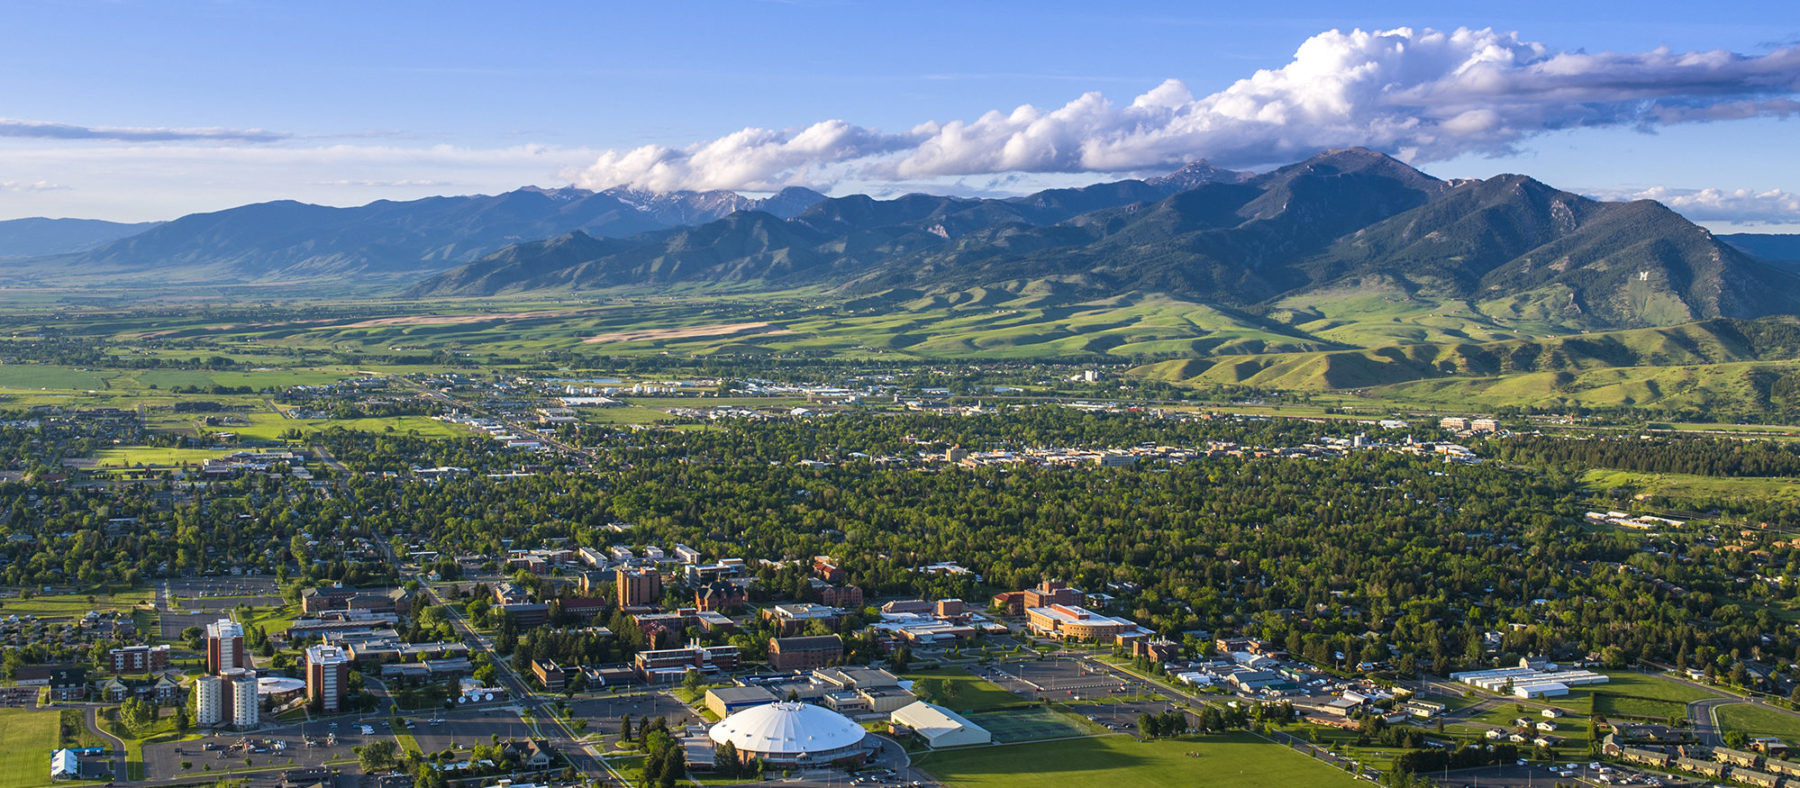
\includegraphics[width=5in,height=\textheight]{images/msu-campus.jpg}
\vspace{1cm}\\
STAT 216 Activity Coursepack}
\usepackage{etoolbox}
\makeatletter
\providecommand{\subtitle}[1]{% add subtitle to \maketitle
  \apptocmd{\@title}{\par {\large #1 \par}}{}{}
}
\makeatother
\subtitle{Fall 2020}
\author{}
\date{\vspace{-2.5em}}

\begin{document}
\maketitle

{
\setcounter{tocdepth}{0}
\tableofcontents
}
\hypertarget{preface}{%
\chapter*{Preface}\label{preface}}
\addcontentsline{toc}{chapter}{Preface}

This coursepack accompanies the textbook for STAT 216: Introduction to Statistics at Montana State University. Each of the activities in this workbook is designed to target specific learning outcomes of the course, giving you practice with important statistical concepts in a group setting with instructor guidance. Bring this workbook with you to class each week, and take notes in the workbook as you would your own notes. A well-written complete workbook will provide an optimal study guide for exams!

\hypertarget{fall-2020-calendar-of-in-class-activities}{%
\chapter*{Fall 2020 Calendar of In-Class Activities}\label{fall-2020-calendar-of-in-class-activities}}
\addcontentsline{toc}{chapter}{Fall 2020 Calendar of In-Class Activities}

\begin{longtable}{|p{.1\textwidth}|l|p{.1\textwidth}|l|p{.40\textwidth}|}
\hline
\textbf{Week}& \textbf{Activity No.}& \textbf{Day}& \textbf{Date}& \textbf{Activity} \\ \hline
\endhead
1& 1& M& 8/17& Martian Alphabet \\*
1& 1& T& 8/18& Martian Alphabet \\*
1& 1& W& 8/19& Martian Alphabet \\*
1& 1& H& 8/20& Martian Alphabet \\*
1& 1& F& 8/21& Martian Alphabet \\ \hline
2& 2& M& 8/24& Study Design \\*
2& 2& T& 8/25& Study Design \\*
2& 2& W& 8/26& Study Design \\*
2& 2& H& 8/27& Study Design \\*
2& 2& F& 8/28& Study Design \\ \hline
3& 3& M& 8/31& Current Population Survey \\*
3& 3& T& 9/1& Current Population Survey \\*
3& 3& W& 9/2& Current Population Survey \\*
3& 3& H& 9/3& Current Population Survey \\*
3& 3& F& 9/4& Current Population Survey \\ \hline
4& -& M& 9/7&	No class $-$ Labor Day \\*
4& 4& T& 9/8& IMDb Movie Reviews: Part I \\*
4& 4& W& 9/9& IMDb Movie Reviews: Part I \\*
4& 4& H& 9/10& IMDb Movie Reviews: Part I \\*
4& 4& F& 9/11& IMDb Movie Reviews: Part I \\ \hline
5& 4& M& 9/14& IMDb Movie Reviews: Part I \\*
5& 5& T& 9/15& IMDb Movie Reviews: Part II \\*
5& 5& W& 9/16& IMDb Movie Reviews: Part II \\*	
5& 5& H& 9/17& IMDb Movie Reviews: Part II \\*
5& 5& F& 9/18& IMDb Movie Reviews: Part II \\ \hline
6& 5& M& 9/21& IMDb Movie Reviews: Part II \\*
6& -& T-F& 9/22-9/25& Exam 1 \\ \hline
7& -& M& 9/28& Exam 1 \\*
7& 6& T& 9/29& Handedness of Male Boxers \\*
7& 6& W& 9/30& Handedness of Male Boxers \\*	
7& 6& H& 10/1& Handedness of Male Boxers \\*
7& 6& F& 10/2& Handedness of Male Boxers \\ \hline
8& 6& M& 10/5& Handedness of Male Boxers \\*
8& 7& T& 10/6& Helmet Use and Head Injuries \\*
8& 7& W& 10/7& Helmet Use and Head Injuries \\*	
8& 7& H& 10/8& Helmet Use and Head Injuries \\*
8& 7& F& 10/9& Helmet Use and Head Injuries \\ \hline
9& 7& M& 10/12& Helmet Use and Head Injuries \\*
9& 8& T& 10/13& COVID-19 and Air Pollution \\*
9& 8& W& 10/14& COVID-19 and Air Pollution \\*	
9& 8& H& 10/15& COVID-19 and Air Pollution \\*
9& 8& F& 10/16& COVID-19 and Air Pollution \\ \hline
10& 8& M& 10/19& COVID-19 and Air Pollution \\*
10& 9& T& 10/20& Record Snowfall \\*
10& 9& W& 10/21& Record Snowfall \\*	
10& 9& H& 10/22& Record Snowfall \\*
10& 9& F& 10/23& Record Snowfall \\ \hline
11& 9& M& 10/26& Record Snowfall \\*
11& 10& T& 10/27& Hand Dexterity \\*
11& 10& W& 10/28& Hand Dexterity \\*	
11& 10& H& 10/29& Hand Dexterity \\*
11& 10& F& 10/30& Hand Dexterity \\ \hline
12& 10& M& 11/2& Hand Dexterity \\*
12& -& T& 11/3& No class  $-$  Election Day \\*
12& -& W-F& 11/4-11/6& Exam 2 \\ \hline
13& -& M-T& 11/9-11/10& Exam 2 \\*
13& -& W& 11/11& No class  $-$  Veterans Day \\*
14& -& H-W&11/12-11/18& Review \\ \hline
\end{longtable}

\hypertarget{martian-alphabet}{%
\chapter{Martian Alphabet}\label{martian-alphabet}}

\hypertarget{learning-outcomes}{%
\section{Learning outcomes}\label{learning-outcomes}}

\begin{itemize}
\item
  Describe the statistical investigation process
\item
  Identify observational units, variables, and variable types in a statistical study
\end{itemize}

\hypertarget{can-you-read-martian}{%
\section{Can you read ``Martian''?}\label{can-you-read-martian}}

How well can humans distinguish one ``Martian'' letter from another? In today's activity, we'll find out. When shown the two Martian letters, Kiki and Bumba, write down whether you think Bumba is on the left or the right.

\vspace{0.5in}

\hypertarget{steps-of-the-statistical-investigation-process}{%
\subsection{Steps of the statistical investigation process}\label{steps-of-the-statistical-investigation-process}}

The first step of any statistical investigation is to ask a research question. In this study the research question is: can we as a class read Martian? (we will refine this later on!). To answer any research question, we must design a study and collect data. (This will normally be provided for you in class.) For our question, the study consists of each student being presented with two Martian letters and asking which was Bumba. Your responses will become our observed data that we will explore. To answer the research question we will simulate what \emph{could} have happened in our class given random chance, repeat that many times to understand the expected variability between different ``randomly guessing'' classes, then comparing our class's observed data to the simulation. This gives us an estimate of how often (or the probability of) our class's result would occur if we were all merely guessing, allowing us to determine if we as a class can in fact read Martian.

Let's explore the data.
\textbf{Observational units} or \textbf{cases} are the subjects data is collected on. In a data set the rows will represent a single observational unit.

\begin{enumerate}
\def\labelenumi{\arabic{enumi}.}
\tightlist
\item
  What are the observational units in this study?
\end{enumerate}

\vspace{0.5in}

\begin{enumerate}
\def\labelenumi{\arabic{enumi}.}
\setcounter{enumi}{1}
\tightlist
\item
  How many students are in class today? This is the sample size.
\end{enumerate}

\vspace{0.5in}

\newpage

A \textbf{variable} is information collected or measured on each observational unit or case. We will look at two types of variables: \textbf{quantitative} and \textbf{categorical}. Each column in a data set will represent a different variable.

Quantitative variables are numerical measurements that can be discrete (whole, non-negative numbers) or continuous (any value within an interval). The number of students in a class would be a discrete variable as you can not have a partial student. GPA would be a continuous variable ranging from 0 to 4.0.

Categorical variables are data that are in groups or categories such as eye color, state of residency, or whether or not a student is considered in-state. Categorical variables with a natural ordering are considered ordinal variables while those without a natural ordering are considered a nominal variable. All variables will be treated as nominal for analysis.

\begin{figure}

{\centering 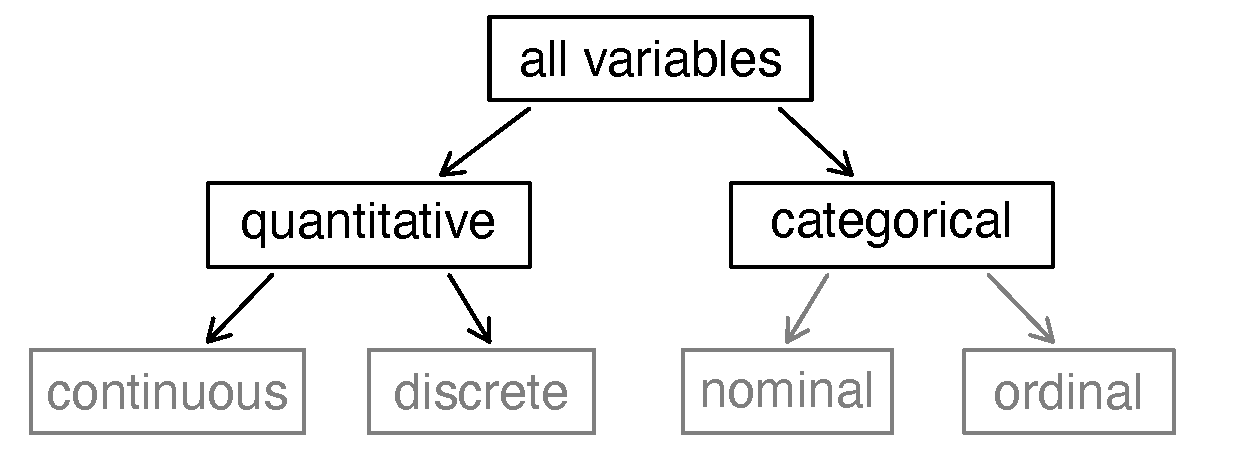
\includegraphics[width=0.75\linewidth]{images/variables} 

}

\caption{Types of variables.}\label{fig:unnamed-chunk-1}
\end{figure}

\begin{enumerate}
\def\labelenumi{\arabic{enumi}.}
\setcounter{enumi}{2}
\tightlist
\item
  Identify the variable we are collecting on each observational unit in this study, i.e., what are we measuring on each student?
\end{enumerate}

\vspace{.8in}

It is important to note that a variable is different than a summary statistic. A variable is measured on a \textbf{single observational unit} while a summary statistic is calculated from a group of observational units. For example, the variable \textbf{whether or not a student is considered in-state} can be measured on each individual student. In a class of 50 students we can calculate the proportion of students who are considered in-state, the summary statistic. Make sure you wrote the variable in question 3 as a variable \textbf{NOT} a summary statistic.

\begin{enumerate}
\def\labelenumi{\arabic{enumi}.}
\setcounter{enumi}{3}
\tightlist
\item
  Is the variable identified in question 3 categorical or quantitative?
\end{enumerate}

\vspace{0.3in}

\begin{enumerate}
\def\labelenumi{\arabic{enumi}.}
\setcounter{enumi}{4}
\tightlist
\item
  Were you correct or incorrect in identifying Bumba?
\end{enumerate}

\vspace{0.3in}

We will now collect the data from the entire class.

\begin{enumerate}
\def\labelenumi{\arabic{enumi}.}
\setcounter{enumi}{5}
\tightlist
\item
  How many people in your class were correct in identifying Bumba? Using the class size from question 2, calculate the proportion of students who correctly identified Bumba.
\end{enumerate}

\begin{center}
$\mbox{proportion} = \frac{\mbox{number of students who correctly identified Bumba}}{\mbox{total number of students}}$
\end{center}

\newpage

Looking at the data set and the summary statistics is only one way to display the data. We will also want to create a visualization or picture of the data. A \textbf{frequency bar plot} is used to display categorical data as a count or frequency. Since our variable has two levels, correct or incorrect, we will create two bars one for each level.

\begin{enumerate}
\def\labelenumi{\arabic{enumi}.}
\setcounter{enumi}{6}
\tightlist
\item
  Plot the observed class data using a frequency bar plot.
\end{enumerate}

\begin{flushleft}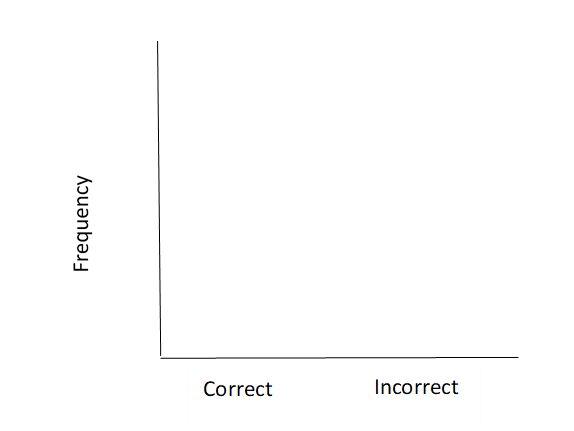
\includegraphics[width=0.75\linewidth]{images/barplot_martian} \end{flushleft}

We can also visualize the data as a proportion in a \textbf{relative frequency bar plot}. Relative frequency is the proportion calculated for each level of the categorical variable.

\begin{enumerate}
\def\labelenumi{\arabic{enumi}.}
\setcounter{enumi}{7}
\tightlist
\item
  Plot the observed class data using a relative frequency bar plot.
\end{enumerate}

\begin{flushleft}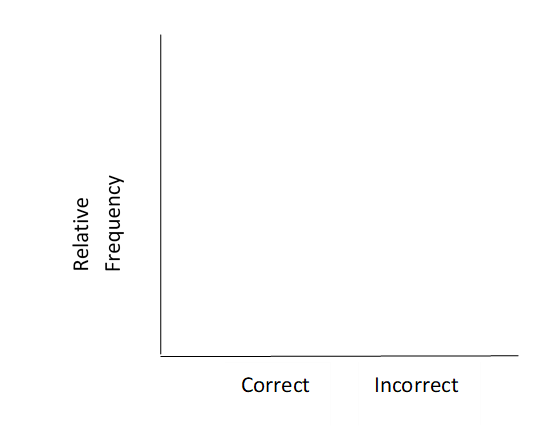
\includegraphics[width=0.75\linewidth]{images/relative_barplot_martian} \end{flushleft}

\newpage

\begin{enumerate}
\def\labelenumi{\arabic{enumi}.}
\setcounter{enumi}{8}
\item
  The next step is to analyze the data. If humans really don't know Martian and are just guessing which is Bumba, what are the chances of getting it right?
  \vspace{0.5in}

  How could we use a coin to simulate each student ``just guessing'' which martian letter is Bumba?
  \vspace{1in}

  How could we use coins to simulate the entire class ``just guessing'' which martian letter is Bumba?
  \vspace{1in}

  How many people in your class would you expect to choose Bumba correctly just by chance? Explain your reasoning.
  \vspace{1in}
\item
  Each of you will flip a coin one time to simulate your ``guess''. Let Heads = correct, Tails = incorrect. What was the result of your simulation?
  \vspace{.4in}

  What was the result from your class's simulation? What proportion of students ``guessed'' correctly in the simulation?
  \vspace{.4in}
\item
  If students really don't know Martian and are just guessing which is Bumba, which seems more unusual: the result from your class's \textbf{simulation} or the observed proportion of students in your class that were correct (this is your data from question 6)? Explain your reasoning.
\end{enumerate}

\newpage

\begin{enumerate}
\def\labelenumi{\arabic{enumi}.}
\setcounter{enumi}{11}
\tightlist
\item
  While your observed class data is likely far different from the simulated ``just-guessing'' class, comparing our class data to a single simulation does not seem to give enough information. The differences seen could just be due to that set of coin flips! Let's simulate another class. Each student should flip your coin again. What was the result from your class's second simulation? What proportion of students ``guessed'' correctly in the second simulation? Create a plot to compare the two simulated results with the observed class result.
\end{enumerate}

\vspace{1in}

\begin{enumerate}
\def\labelenumi{\arabic{enumi}.}
\setcounter{enumi}{12}
\tightlist
\item
  We still unfortunately only have a couple of simulations to compare our class data to. It would be much better to be able to see how our class compared to hundreds or thousands of ``just-guessing'' classes. Since we don't want to flip coins all class period, your instructor will use a computer simulation to get 1000 trials. Fill in the following blanks to describe how we would create a simulation of random guessing with 1000 trials.
\end{enumerate}

~~~~~~~~~~Probability of correct guesses: \_\_\_\_\_

\vspace{0.1in}

~~~~~~~~~~Sample size: \_\_\_\_\_

\vspace{0.1in}

~~~~~~~~~~Number of repetitions: \_\_\_\_\_

\vspace{0.1in}

\begin{enumerate}
\def\labelenumi{\arabic{enumi}.}
\setcounter{enumi}{13}
\tightlist
\item
  Sketch the distribution displayed by your instructor here, being sure to label each axis appropriately.
\end{enumerate}

\vspace{2in}

\begin{enumerate}
\def\labelenumi{\arabic{enumi}.}
\setcounter{enumi}{14}
\tightlist
\item
  Is your class particularly good or bad at Martian? How can you use the plot in question 14 to tell?
\end{enumerate}

\vspace{1in}

\begin{enumerate}
\def\labelenumi{\arabic{enumi}.}
\setcounter{enumi}{15}
\tightlist
\item
  Is it \emph{possible} that we could see our class results just by chance if everyone was just guessing? Explain your reasoning.
\end{enumerate}

\vspace{1in}

\begin{enumerate}
\def\labelenumi{\arabic{enumi}.}
\setcounter{enumi}{16}
\tightlist
\item
  Is it \emph{likely} that we could see our class results just by chance if everyone was just guessing? Explain your reasoning.
\end{enumerate}

\vspace{1in}

\begin{enumerate}
\def\labelenumi{\arabic{enumi}.}
\setcounter{enumi}{17}
\tightlist
\item
  Does this activity provide strong evidence that students were not just guessing at random? If so, what do you think is going on here? Can we as a class read Martian?
\end{enumerate}

\vspace{1in}

\hypertarget{take-home-messages}{%
\section{Take home messages}\label{take-home-messages}}

\begin{enumerate}
\def\labelenumi{\arabic{enumi}.}
\item
  In this course we will learn how to evaluate a claim by comparing observed results (classes' ``guesses'') to a distribution of many simulated results under an assumption like ``blind guessing.''
\item
  Blind guessing between two outcomes will be correct only about half the time. We can create data (via computer simulation) to fit the assumption of blind guessing.
\item
  Unusual observed results will make us doubt the assumptions used to create the simulated distribution. A large number of correct ``guesses'' is evidence that a person was not just blindly guessing.
\end{enumerate}

\hypertarget{additional-notes}{%
\section{Additional notes}\label{additional-notes}}

Use this space to summarize your thoughts and take additional notes on today's activity, and to write down the names and contact information of your team mates.

\hypertarget{study-design}{%
\chapter{Study Design}\label{study-design}}

\hypertarget{learning-outcomes}{%
\section{Learning outcomes}\label{learning-outcomes}}

\begin{itemize}
\item
  Explain the purpose of random sampling and its effect on scope of inference
\item
  Explain the purpose of random assignment and its effect on scope of inference
\item
  Identify whether a study is observational or an experiment
\item
  Identify confounding variables in observational studies and explain why they are confounding
\item
  Identify the types of bias present in a study
\end{itemize}

\hypertarget{terminology-review}{%
\section{Terminology review}\label{terminology-review}}

Statistics is the study of how best to collect, analyze, and draw conclusions from data. Statistical inference will allow us to make a statement about a population parameter based on a sample statistic.

Some terms covered in this activity are\ldots{}

\begin{itemize}
\item
  Population
\item
  Sample
\item
  Parameter
\item
  Statistic
\item
  Selection Bias
\item
  Response Bias
\item
  Non-response Bias
\item
  Scope of Inference
\item
  Explanatory Variable
\item
  Response Variable
\item
  Confounding Variable
\item
  Experiments
\item
  Observational Study
\end{itemize}

To review these concepts see Section 1.3 to 1.6 in the textbook.

\newpage

\hypertarget{types-of-sampling-bias}{%
\section{Types of sampling bias}\label{types-of-sampling-bias}}

There are two parts to study design: how the sample was selected and how the study was conducted. First we will look at sampling and types of bias.

In these next questions, identify the target population, the sample, the variable, and the type of bias present.

\begin{enumerate}
\def\labelenumi{\arabic{enumi}.}
\item
  To determine if the proportion of out of state undergraduate students at Montana State University has increased in the last 10 years, a statistics instructor sent an email survey to 500 randomly selected current undergraduate students. One of the questions on the survey asked whether they had in-state or out-of-state residency. She only received 378 responses.
  \vspace{0.25in}

  Target population:
  \vspace{0.3in}

  Sample:
  \vspace{0.3in}

  Variable:
  \vspace{0.3in}

  Type of Bias:
  \vspace{0.3in}
\item
  PEW Research surveys US adults about many different topics. Recently a survey was conducted to assess current presidential approval. A random sample of 6395 US adults was taken. Of those surveyed, 42\% say they agree with President Trump on many or nearly all of the top issues facing the country today.
  \vspace{0.25in}

  Target population:
  \vspace{0.3in}

  Sample:
  \vspace{0.3in}

  Variable:
  \vspace{0.3in}

  Type of Bias:
  \vspace{0.3in}
\end{enumerate}

\newpage

\begin{enumerate}
\def\labelenumi{\arabic{enumi}.}
\setcounter{enumi}{2}
\item
  A television station is interested in predicting whether or not voters in its listening area are opposed to legalizing marijuana for adult use. It asks its viewers to phone in and indicate whether they are in favor of this or opposed to this. Of the 2241 viewers who phoned in, forty-five percent were opposed to legalizing marijuana.
  \vspace{0.1in}

  Target population:
  \vspace{0.3in}

  Sample:
  \vspace{0.3in}

  Variable:
  \vspace{0.3in}

  Type of Bias:
  \vspace{0.3in}
\item
  To gauge the interest in a new swimming pool, a local organization stood outside of the Bogart Pool during open hours. One of the questions they asked was, ``Since the Bogart Pool is in such bad repair, don't you agree that the city should fund a new pool?''
  \vspace{0.1in}

  Target population:
  \vspace{0.3in}

  Sample:
  \vspace{0.3in}

  Variable:
  \vspace{0.3in}

  Type of Bias:
  \vspace{0.3in}
\item
  The Bozeman school district is interested in surveying parents of students about their opinions on returning to school this fall following the COVID-19 pandemic. They divided the school district into 10 divisions based on location and randomly surveyed 20 households within each division.
  \vspace{0.1in}

  Target population:
  \vspace{0.3in}

  Sample:
  \vspace{0.3in}

  Variable:
  \vspace{0.3in}

  Type of Bias:
  \vspace{0.3in}
\end{enumerate}

\newpage

\hypertarget{study-design-1}{%
\section{Study design}\label{study-design-1}}

The two main study designs we will cover are observational studies and experiments. Both the sampling method and the study design will help to determine the \textbf{scope of inference} for a study. Remember that only in a randomized experiment can we conclude a \textbf{causal} (cause and effect) relationship between the explanatory and response variable.

\begin{center}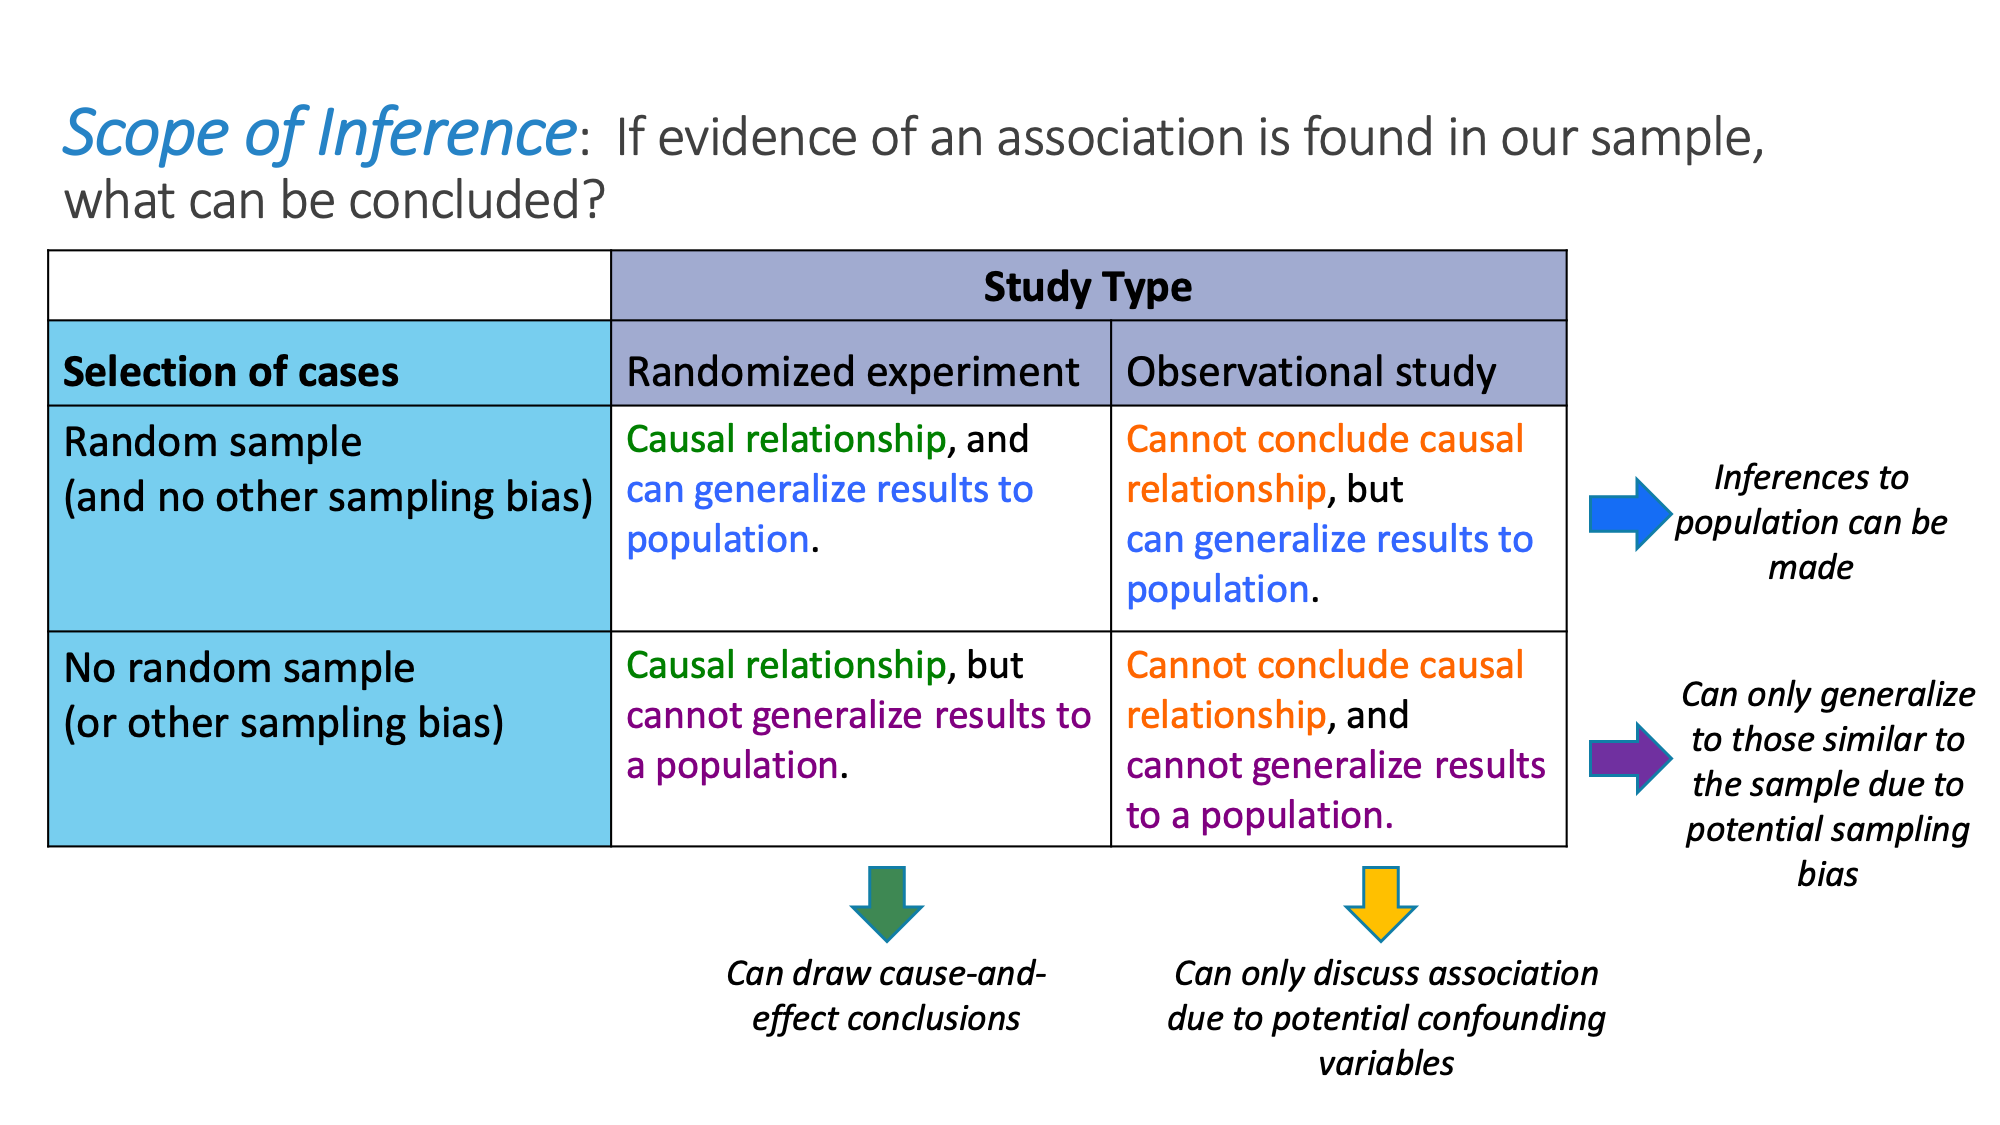
\includegraphics[width=0.75\linewidth]{images/ScopeOfInference} \end{center}

For the next exercises, identify the explanatory variable, the response variable, a potential confounding variable, and the study design.

\begin{enumerate}
\def\labelenumi{\arabic{enumi}.}
\setcounter{enumi}{5}
\item
  The pharmaceutical company, Moderna Therapeutics is working in conjunction with the National Institute of Health towards a vaccine for COVID-19 and has recently begun Phase 3 clinical trials. US Clinical research sites will enroll 30,000 volunteers without COVID-19 to participate. Participants will be randomly assigned to receive either the candidate vaccine or a saline placebo. They will then be followed to assess vaccine related symptoms and development of COVID-19. The trial is blinded, so the investigators and the participants will not know who is assigned to which group.
  \vspace{0.25in}

  Explanatory Variable:
  \vspace{0.25in}

  Response Variable:
  \vspace{0.25in}

  Confounding Variable:
  \vspace{0.25in}

  Study design:
  \vspace{0.25in}

  What is the scope of inference for this study?
  \vspace{0.5in}
\item
  In another study, a local health department randomly selected 1000 US adults without COVID-19 to participate in a health survey. Each participant was assessed at the beginning of the study and then followed for 1 year. They were interested to see which participants elected to receive a vaccination for COVID-19 and whether any participants developed COVID-19.
  \vspace{0.25in}

  Explanatory Variable:
  \vspace{0.25in}

  Response Variable:
  \vspace{0.25in}

  Confounding Variable:
  \vspace{0.25in}

  Study design:
  \vspace{0.25in}

  What is the scope of inference for this study?
  \vspace{0.5in}
\item
  What is a potential confounding variable for the study in question 7? Explain how this meets the definition of a confounding variable.
  \vspace{1in}
\end{enumerate}

\hypertarget{additional-notes}{%
\section{Additional notes}\label{additional-notes}}

Use this space to summarize your thoughts and take additional notes on today's activity.

\end{document}
